\chapter{Описание АСУ ТП для СК}\label{ch:chn}

\section{Общие слова. Введение в тему}

% https://m.studref.com/495961/ekonomika/klassifikatsiya_imitatsionnyh_modeley_promyshlennogo_predpriyatiya

Автоматизированная система управления технологическим процессом (АСУ ТП) --- это термин,
имеющий отношение к ЭВМ, обеспечивающим управление различными техническими процессами \cite{journal:iter_research_guriev_2016}.
Изначально системы АСУ~ТП использовались исключительно на производстве, но с развитием технологий
и из-за сходства технических процессов АСУ~ТП вышло за рамки управления сугубо производственными процессами
и перешла в другие сферы деятельности, от управления транспортом %\cite{}
до управления техническими процессами зданий \cite{journal:vechisl_tech:2013:Golushko}
и более сложными техническими сооружениями (например, здесь \cite{journal:vechisl_tech:2004_okolnischnikov}).
%
Далее будет показано создание \todo{аналитической} модели объекта контроля
при создании имитатора объекта контроля и его применение на всех этапах жизненного цикла
объекта контроля: от постановки задачи и проектирования системы контроля, до пусконаладочных работ
и сдачи в опытную эксплуатацию.


Стоит отметить, что для более качественной/глубокой имитации необходимо выделять несколько моделей
(которые по факту являются подмоделями, но так как они могут выступать в качестве самостоятельных единиц исследования,
далее будем называть их моделями),
анализируя данные этих моделей (экспериментально) установить свойства этих моделей:
стационарность, детерминированность и проч.

В модели объекта контроля может быть несколько моделей \cite{journal:vechisl_tech:2004_okolnischnikov}:
\begin{itemize}
    \item модель технологического объекта управления (правила перехода);
    \item модель имитации внешних сигналов;
    \item модель внутреннего состояния объекта контроля (токи, напряжения и т.д. и т.п.);
    \item \ldots
\end{itemize}

Для пояснения смотри рисунок \ref{fig:submodels_asu_tp}.

\begin{center}
    \begin{figure}[hb]
        % \includegraphics[width=.8\textwidth]{submodels_asu_tp}
        \caption{Структура модели}\label{fig:submodels_asu_tp}
    \end{figure}
\end{center}

Поскольку построение чисто аналитической модели имеет недостаток  в виде отсутствия возможности
описать поведение исследуемого объекта во времени, используется имитационная модель.

\textit{Имитационное моделирование} --- процесс построения некоего алгоритма, который имитирует
поведение исследуемого объекта и взаимодействие исходного объекта с учетом возможных случайных входных величин и
воздействий из внешней среды \cite{book:vvedeni_imit_model_1987}.

Объекты контроля, такие как
    необитаемые автономные подводные аппараты \todo{\ldots},
на которые в любой момент времени возлагается функция готовности к  работе,
нуждаются в проведении проверок при эксплуатации и хранении.
	%
Для проверки ОК необходима система контроля. Создание и отладка СК сопряжена со следующими факторами.
	%
\begin{itemize}
    \item Дороговизна и труднодоступность достаточного количества статистического материала
    натурных испытаний для отладки алгоритмов ПО СК экономически нецелесообразна, так же связана с риском для жизни испытующих.
    %
    \item ОК находится на этапе проектирования.
    %
    \item Отсутствует возможность подключения к ОК.
    %
    \item Проверка граничных значений алгоритмов ОК, ведущих к разрушению ОК недопустима.
\end{itemize}



\section{Направление информационных потоков} %\label{ch:ch2}

Структурная схема системы контроля показана на рисунке \ref{fig:asc_schema}.
Взаимодействие между каждыми узлами опосредованно, то есть
оператор (диспетчер) взаимодействует с автоматизированным рабочим местом (АРМ),
физическая реализация которого это ЭВМ со специализированным программным обеспечением.
Оператор, выбирая один из режимов работы, сообщает посредством АРМ,
какой набор выходных параметров должна сформировать СК, чтобы объект контроля вышел на заданный режим проверки.
Штрих пунктиром показано взаимодействие оператора с объектом контроля,
которое подразумевает механическое задействование органов управления ОК
или, некий, например, аудио-визуальный контроль состояния узлов ОК.

\begin{center}
    \begin{figure}[hb]
        % 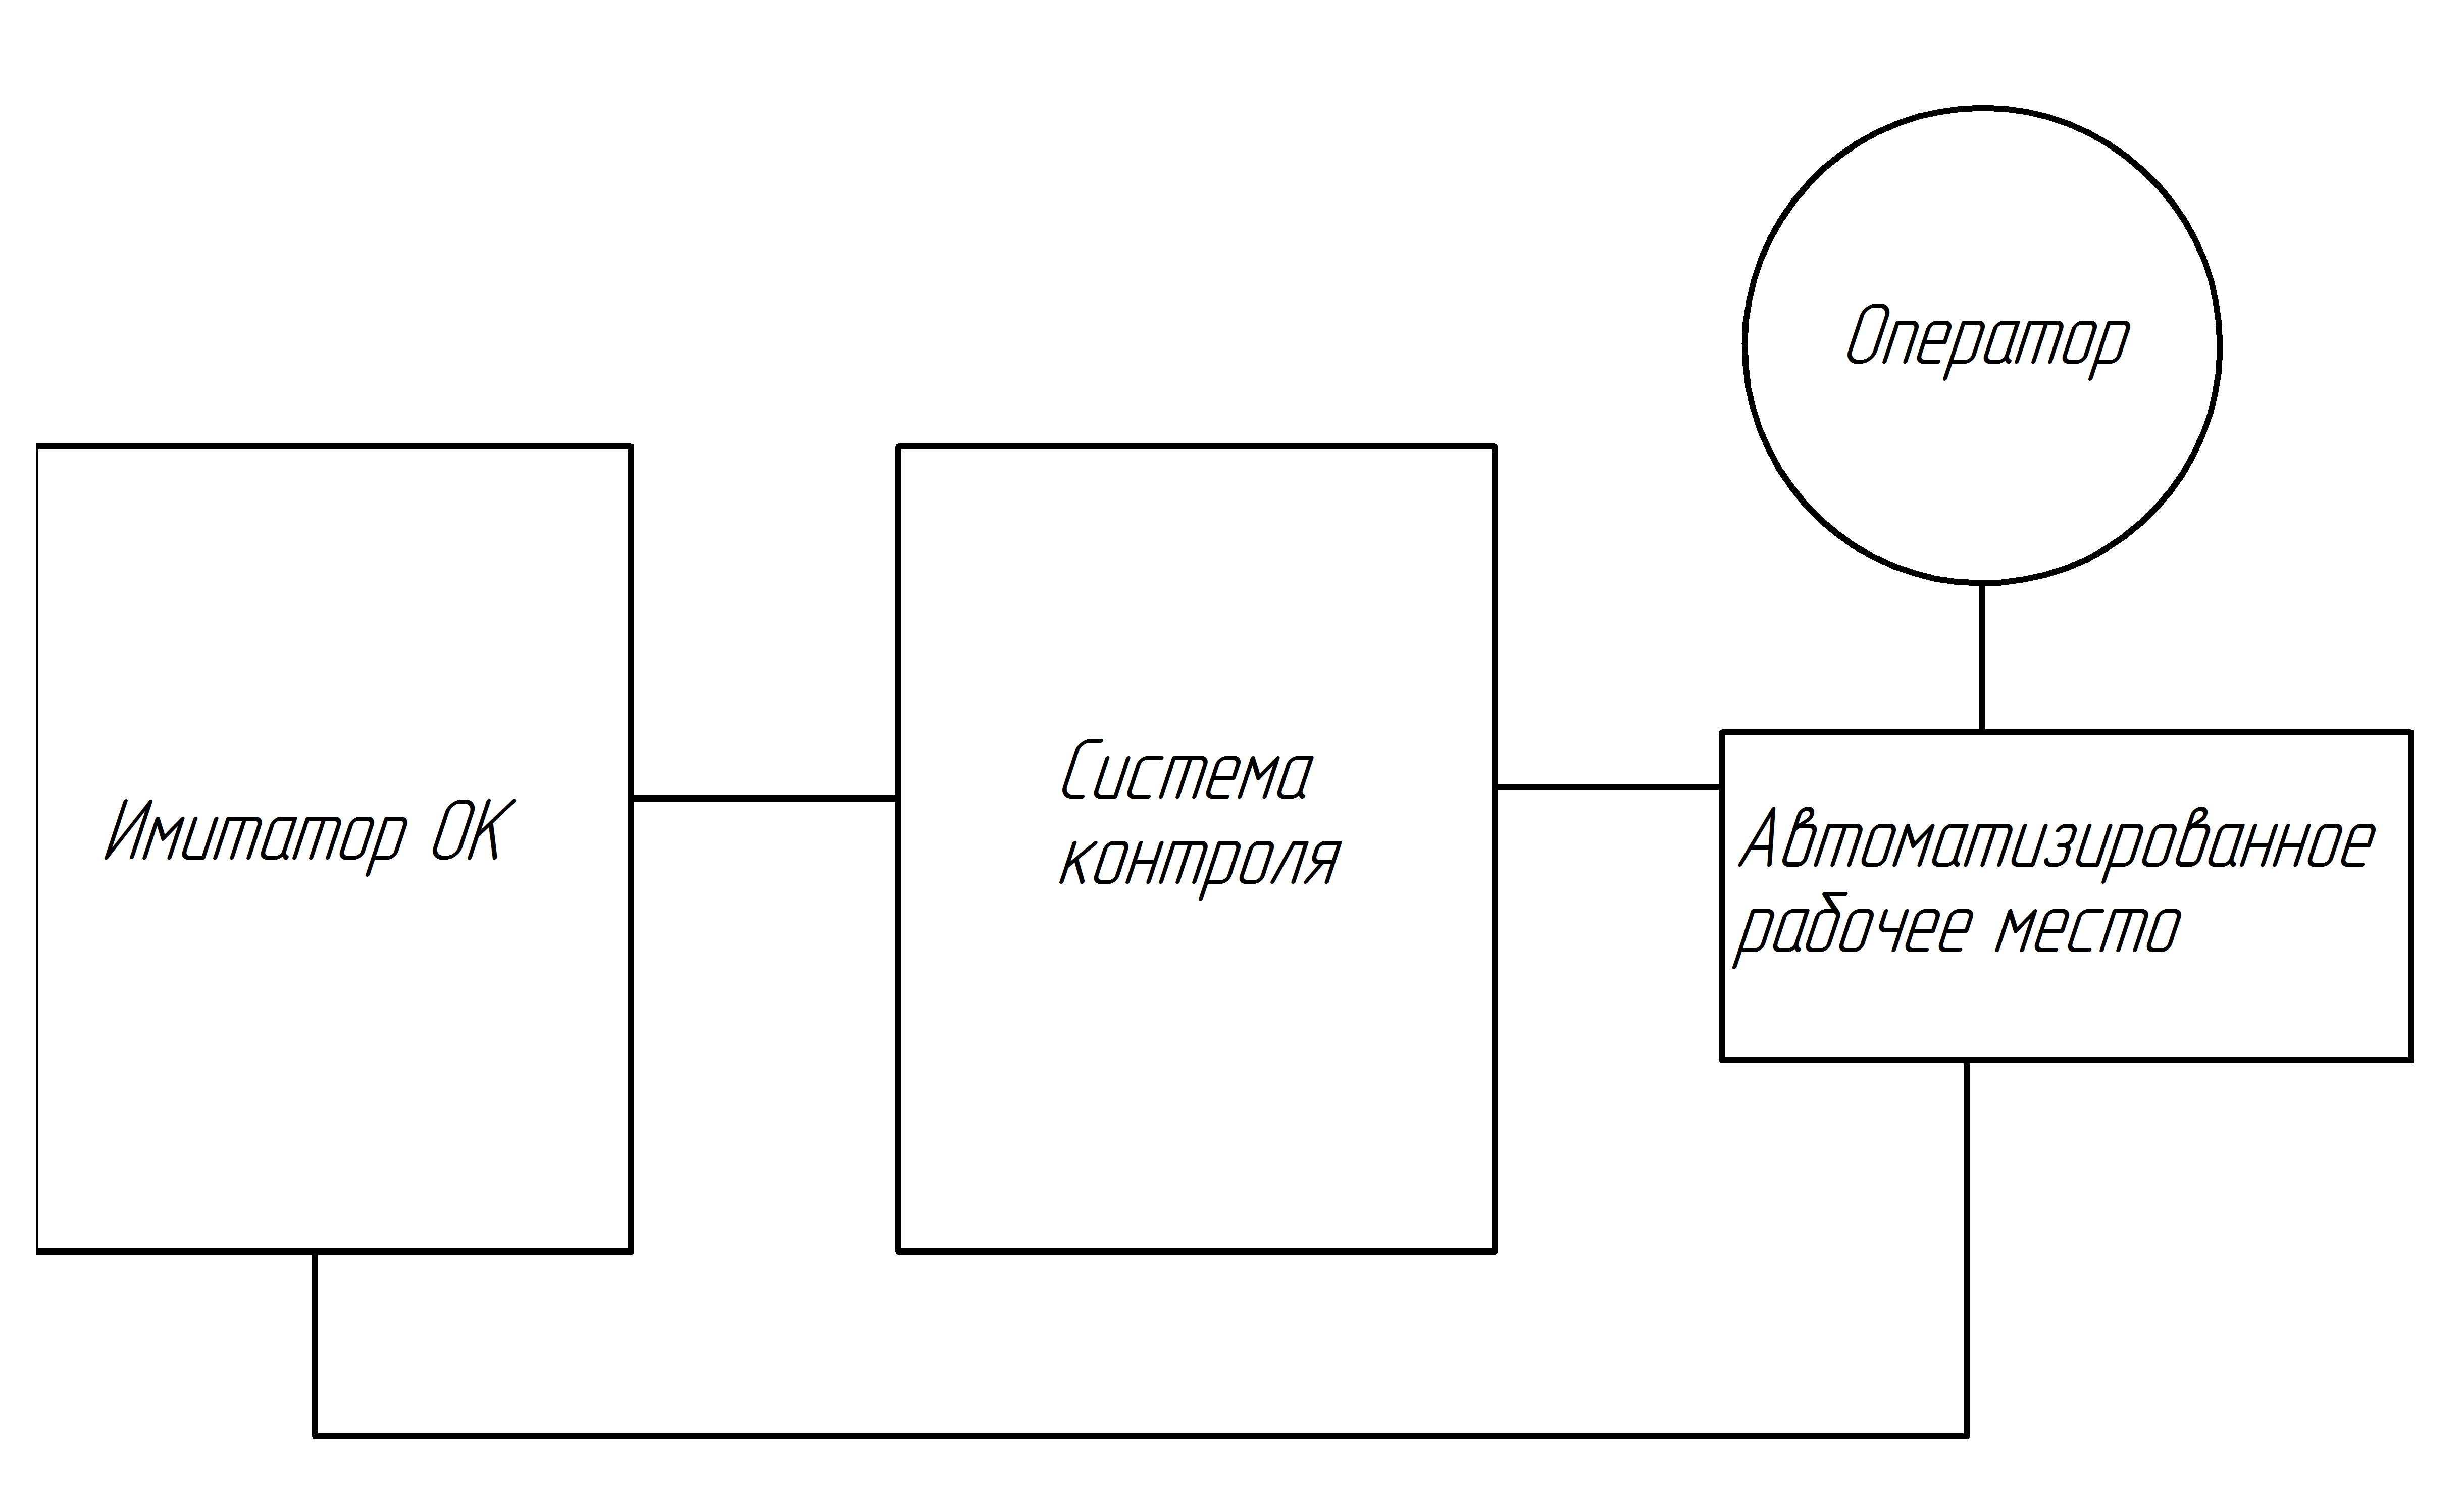
\includegraphics[width=.8\textwidth]{scheme.png}
        \caption{Структура программно-технологического комплекса системы контроля}\label{fig:asc_schema}
    \end{figure}
\end{center}

Более детальное описание информационных потоков показано на рисунке \ref{fig:asc_info_bus}.
Выделяется три уровня: нижний, средний и верхний.

На нижнем уровне располагаются подключаемые по промышленным каналам связи различные приборы, датчики и агрегаты,
которые непосредственно двунаправленно взаимодействуют с ОК, посылая и принимая от него сигналы.
% Так же на этом уровне располагаются прочие устройства, обеспечивающие непосредственное ...

Средний уровень отвечает за обмен информацией между нижним и верхним уровнями. Этот уровень, как правило,
состоит из программируемого логического контроллера (ПЛК). ПЛК реализует различные алгоритмы управления,
осуществляется формирование, сортировка, масштабирование и подготовка данных для передачи между уровнями.
В частности, это может быть осуществлено с помощью блока гальванической развязки (БГР).

Верхний уровень отвечает за графическое представление данных (в широком смысле этого слова),
обеспечивает диспетчеризацию и сбор подготовленных данных посредством человеко-машинного интерфейса.

\begin{center}
    \begin{figure}[hb]
        % 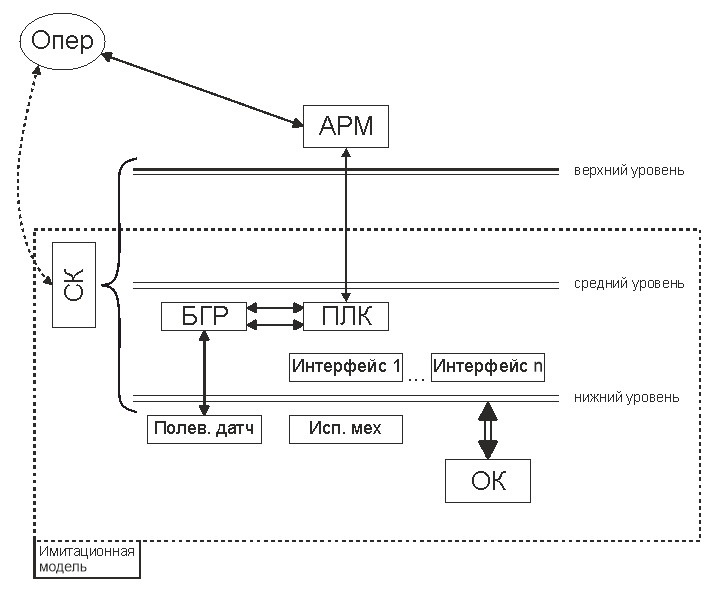
\includegraphics[width=.8\textwidth]{scheme_3levels.png}
        \caption{Информационные шины системы контроля}\label{fig:asc_info_bus}
    \end{figure}
\end{center}

На рисунке \ref{fig:asc_info_bus} штрихом выдела область данных, которая \textit{может быть}
представлена (заменена) имитационное моделью.

Стоит отметить, что в некоторой литературе средний и нижний уровни объединены в один нижний уровень.

\section{Составные части имитационной модели}




% \section{Распределение ролей}
% На стороне СК создается экземпляр клиента сети modbus,
% имитатор представляет сервер (см. главу \ref{ch:ch2}).
% \section{Конфигурационный файл}\label{sec:ch2/sec1}
% Общее пространство данных modbus у ПО СК и имитатора \ldots
% \section{Паттерн MVC}
% Поверх множества данных modbus используется паттерн проектирования модель-вид-контроллер \cite{book:pattern:band_of_4}.
% Библиотека Qt позволяет создавать модель данных, наследуя поведение от \lstinline[language=C]!QAbstractTableModel!,
% переобпределяя реализацию методов для чтения-записи данных в модель.
% \subsection{Пояснение в реализации методов}
% \subsection{Преимущества такого подхода}
